\chapter{Fundamentação Teórica}

\section{Inversor Ponte Completa Bidirecional}

O inversor é um dispositivo capaz de alterar uma tensão de entrada CC e transformá-la em uma tensão de saída CA simétrica, com amplitude e frequência desejadas. Para o caso particular em que a tensão de entrada CC é fixa e não controlável, uma tensão de saída variável é obtida através do controle da modulação por largura de pulso (PWM) do inversor. Os inversores podem ser classificados em monofásicos e trifásicos e estes operam com dispositivos de chaveamento da tensão de entrada (com o uso de BJTs, MOSFETs, IGBTs e outros) \cite{MRashid}. No caso particular deste trabalho, foi utilizado um módulo inversor trifásico com IGBTs - \textit{Insulated Gate Bipolar Transistors} - para realização do chaveamento. 

A composição da unidade inversora utilizada pode ser visualizada na Fig. \ref{fig:Inversor}.

\begin{figure}[!hbt]
	% Center the figure.
	\begin{center}
		% Include the eps file, scale it such that it's width equals the column width. You can also put width=8cm for example...
		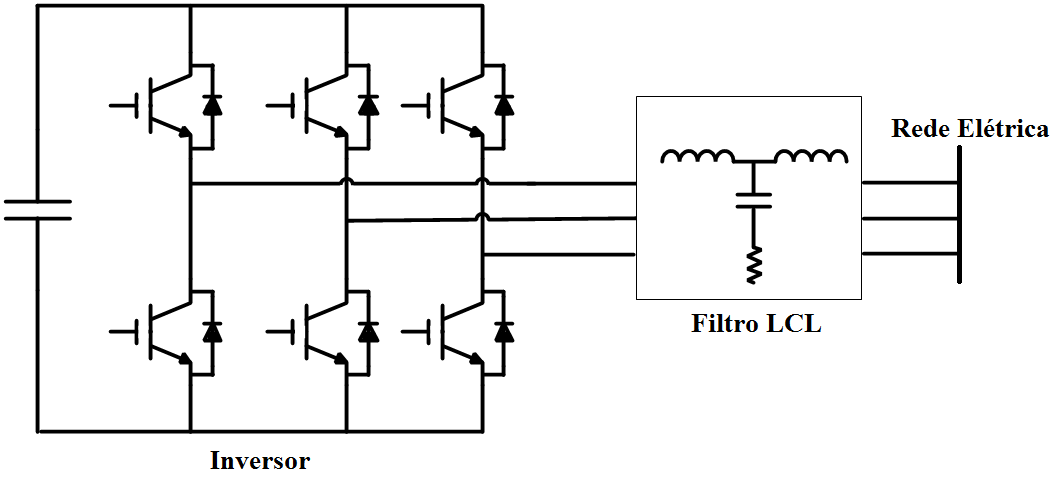
\includegraphics[scale=0.5]{figuras/Inversor.png}
		% Create a subtitle for the figure.
		\caption{Topologia do inversor utilizado e filtro de conexão. Fonte: Autor.}
		% Define the label of the figure. It's good to use 'fig:title', so you know that the label belongs to a figure.
		\label{fig:Inversor}
	\end{center}
\end{figure}


\section{Filtro LCL}

A utilização da modulação por largura de pulso (PWM) em conjunto com uma malha fechada de controle de corrente pode ocasionar harmônicos de alta ordem que levam a distúrbios em equipamentos ligados a rede, e desta forma, produzir perdas. Para que estes harmônicos próximos à frequência de chaveamento sejam reduzidos, um valor alto de impedância deve ser utilizado. Porém, para aplicações que exigem alta potência, na ordem de alguns quilowatts, esta estratégia se torna altamente dispendiosa, e além disso, a resposta dinâmica final do sistema pode piorar, conforme define \cite{1510826}.

Como alternativa, surge a topologia de filtro LCL mostrado na Fig. \ref{fig:Filtro-LCL}. O sistema de filtragem empregado consiste, basicamente, de uma associação de dois conjuntos de indutores e um capacitor em paralelo. Este conjunto tem por funções básicas garantir, na frequência fundamental, um comportamento indutivo na saída do inversor, e ainda, a atenuação das componentes harmônicas de alta frequência produzidas pelo PWM. 

\begin{figure}[!hbt]
	% Center the figure.
	\begin{center}
		% Include the eps file, scale it such that it's width equals the column width. You can also put width=8cm for example...
		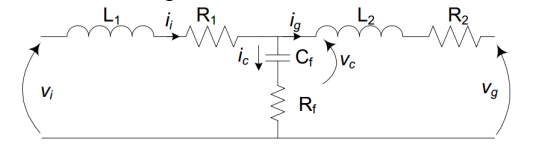
\includegraphics[width=\columnwidth]{figuras/Filtro_LCL.PNG}
		% Create a subtitle for the figure.
		\caption{Modelo de filtro LCL por fase. Fonte: \cite{ReznikSimoes2014}}
		% Define the label of the figure. It's good to use 'fig:title', so you know that the label belongs to a figure.
		\label{fig:Filtro-LCL}
	\end{center}
\end{figure}

Destaca-se que o filtro em pauta possui seus parâmetros definidos com base na metodologias apresentadas em \cite{1510826} e \cite{ReznikSimoes2014}, a qual consideram que:

\begin{itemize}
	\item Os indutores são definidos com o objetivo de mitigar o \textit{ripple} de corrente produzido pelo chaveamento do inversor;
	\item Os capacitores são escolhidos para que na frequência fundamental haja fornecimento de potência reativa à rede elétrica, de forma que o capacitor $C_f$ definido na Figura \ref{fig:Filtro-LCL} não possa ultrapassar 5\% deste valor;
	\item A queda de tensão admissível nos indutores do filtro, quando do fornecimento da potência nominal da unidade aerogeradora, deverá estar limitada a 0,1 pu;
	\item A frequência de ressonância dos componentes, devido ao filtro escolhido, deve estar na faixa definida pela Eq. \ref{eq:frequencia_ressonancia}.
	
\begin{align}\label{eq:frequencia_ressonancia}
10 \omega_{rede} \leq \omega_{ressonância} \leq \omega_{chaveamento}
\end{align}
	\item A resistência para amortecimento da ressonância é calculada em função da impedância do capacitor na frequência de ressonância.
\end{itemize}
	

O valor de impedância do sistema é calculado pela Eq. \ref{eq:impedancia_sistema}, onde $V_n$ refere-se à tensão nominal do sistema e $S_n$ à potência aparente total do sistema.

\begin{align}\label{eq:impedancia_sistema}
	Z_b = \frac{V_n^2}{S_n}
\end{align}

Tendo em vista os critérios definidos, as seguintes etapas devem ser seguidos para a definição dos parâmetros do filtro LCL:

\begin{enumerate}
	\item \textbf{Indutor do lado do inversor}: este elemento é calculado através da Eq. \ref{eq:indutor_L1}, considerando que valores típicos para o \textit{ripple} de corrente no indutor do lado do conversor estão na ordem de 10 a 25\%, onde $V_f$ refere-se à tensão da rede, $f_{sw}$ à frequência de chaveamento, e $i_{ripple}$ ao \textit{ripple} máximo de corrente do lado do inversor.

	\begin{align}\label{eq:indutor_L1}
		L_1 = \frac{V_f}{2\sqrt{6}f_{sw}i_{ripple}}
	\end{align}
	
	\item \textbf{Capacitância}: Como já exposto acima, a capacitância deve ser encontrada a partir do valor máximo de potência reativa que deve ser fornecida na frequência fundamental, conforme a Eq. \ref{eq:capacitancia_fundamental}.
	
	\begin{align}\label{eq:capacitancia_fundamental}
		C_f = \frac{Q_C}{\omega_{rede}V^2_n}
	\end{align}
	
	\item \textbf{Indutor do lado da rede}: O indutor do lado da rede é determinado a partir da constante \textit{r}, a qual é calculada como uma função dos parâmetros $L_1$, $C_f$ e do \textit{ripple} da corrente injetada na rede elétrica. O \textit{ripple} de saída é definido pela Eq. \ref{eq:ripple_saida} e o indutor do lado da rede, $L_2$, pela Eq. \ref{indutor_lado_rede}.
	
	\begin{align}\label{eq:ripple_saida}
		\frac{i_{rede}}{i_{ripple}} = \frac{1}{|1 + r(1 - L_1C_f(2\pi f_{sw})^2)|}
	\end{align}
	\begin{align}\label{indutor_lado_rede}
		L_2 = rL_1
	\end{align}
	
	\item \textbf{Frequência de ressonância:} a frequência de ressonância do filtro é encontrada por \ref{eq:freq_ressonancia}.
	
	\begin{align}\label{eq:freq_ressonancia}
		\omega_{ressonancia} = \sqrt{\frac{L_1 + L_2}{L_1L_2C_f}}
	\end{align}
	
	\item \textbf{Resistência de amortecimento:} a resistência de amortecimento é determinada como sendo um terço da impedância do capacitor na frequência de ressonância, conforme \ref{eq:resistencia-amortecimento}.
	
	\begin{align}\label{eq:resistencia-amortecimento}
		R_f = \sqrt{\frac{1}{3\omega_{res}C_f}}
	\end{align}
	
\end{enumerate}

\section{Estratégia de Controle}

Haja vista que um conversor de tensão é utilizado, o ajuste do fluxo de potência entre o elemento gerador e a rede elétrica é feito através do controle de corrente produzido pelo inversor, com base em \cite{TeseProfAlex}. A referência cita ainda que, para que se possa obter o controle da corrente de saída, é necessário que se atue sobre a amplitude e ângulo de fase das tensões trifásicas sintetizadas nos terminais de saída do inversor. A Fig. \ref{fig:Estrategia-controle-inversor} apresenta a topologia utilizada para controle do dispositivo.

\begin{figure}[!hbt]
	% Center the figure.
	\begin{center}
		% Include the eps file, scale it such that it's width equals the column width. You can also put width=8cm for example...
		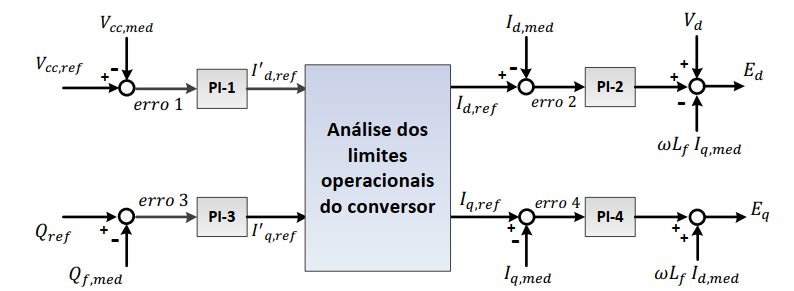
\includegraphics[width=\columnwidth]{figuras/Estrategia_Controle_Inversor.PNG}
		% Create a subtitle for the figure.
		\caption{Estrutura básica de controle da unidade inversora. Fonte: \cite{TeseProfAlex}}
		% Define the label of the figure. It's good to use 'fig:title', so you know that the label belongs to a figure.
		\label{fig:Estrategia-controle-inversor}
	\end{center}
\end{figure}

Pode-se verificar, através da Fig. \ref{fig:Estrategia-controle-inversor}, que deve-se definir um valor de referência para a tensão no barramento de corrente contínua $V_{CC,ref}$. Este sinal é posteriormente comparado com a mesma grandeza medida denominada $V_{CC,med}$, e um valor de erro é gerado. Este erro é o sinal de entrada do controlador PI-1, responsável por fornecer o valor de referência de corrente de eixo direto $I'_{d,ref}$ a ser sintetizado pela unidade inversora. Este mesmo procedimento ocorre na malha de potência reativa, de forma que são comparados os valores de referência $Q_{ref}$ e medido $Q_{f,med}$ e, como resultado, o sinal de erro é enviado para o controlador PI-3, gerando o sinal de referência inicial para a corrente de eixo em quadratura $I'_{q,ref}$.

Visto que as referências de corrente de eixo direto e de eixo em quadratura são produzidas pela unidade inversora, é necessário certificar que os valores obtidos não implicam na violação das capacidades de operação do módulo. Desta forma, estas referências são enviadas ao bloco identificado na Fig. \ref{fig:Estrategia-controle-inversor} como "Análise dos limites operacionais da unidade inversora", que tem como objetivos:

\begin{itemize}
	\item Verificar se as referências calculadas pelos controladores PI-1 e PI-3 não provocam uma ultrapassagem dos valores nominais do inversor, conforme a inequação \ref{eq:analise_limites_operacionais}, onde $S_{\textrm{nominal}}$ e $V_{\textrm{nominal}}$ correspondem, respectivamente, a potência e tensão nominal da unidade inversora.
	
	\begin{align}\label{eq:analise_limites_operacionais}
	{I'_{d,ref}}^2 + {I'_{d,ref}}^2 \leq \frac{\sqrt{2}S_{\textrm{nominal}}}{\sqrt{3}V_{\textrm{nominal}}}
	\end{align}
	
	\item Definir a prioridade operacional, no caso em que as referências iniciais impliquem na ultrapassagem da capacidade nominal da unidade inversora. Assim, o valor de referência da corrente de eixo em quadratura é conservado, permitindo que a tensão no barramento de corrente contínua e o fornecimento de potência ativa se mantenham constantes em detrimento de uma redução na corrente de eixo em quadratura. Este procedimento é mostrado na Fig. \ref{fig:Mecanisco_Sobrecarga}.
	
	\begin{figure}[!hbt]
		% Center the figure.
		\begin{center}
			% Include the eps file, scale it such that it's width equals the column width. You can also put width=8cm for example...
			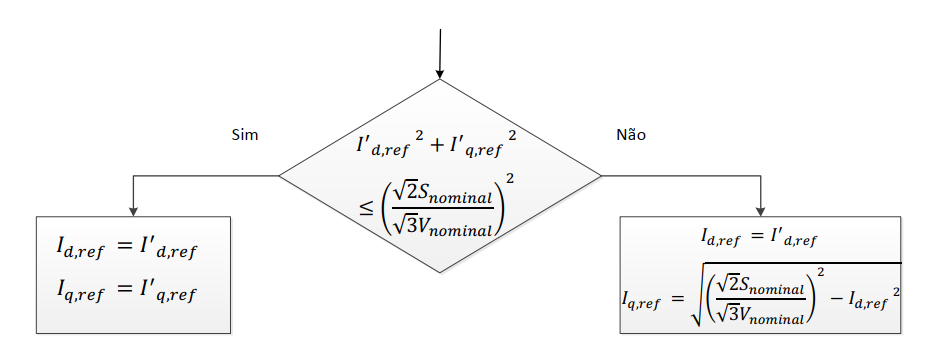
\includegraphics[width=\columnwidth]{figuras/Mecanisco_Sobrecarga.PNG}
			% Create a subtitle for the figure.
			\caption{Tomada de decisão do algoritmo de controle em casos de sobrecarga. Fonte: \cite{TeseProfAlex}}
			% Define the label of the figure. It's good to use 'fig:title', so you know that the label belongs to a figure.
			\label{fig:Mecanisco_Sobrecarga}
		\end{center}
	\end{figure}
	
	\item Por fim, incorporar uma malha denominada \textit{anti windup}, de forma que o comportamento de integração dos controladores PI-1 e PI-3 seja interrompido quando o conversor atingir as condições de saturação. A metodologia utilizada baseia-se no \textit{anti windup back calculation}, conforme \cite{astrom2006advanced}. O diagrama esquemático para a malha referente ao controle de tensão no barramento de corrente contínua está explicitado na Fig. \ref{fig:Malha_anti_windup}. O ajuste do fluxo de potência reativa também segue uma estrutura similar. 
	
	\begin{figure}[!hbt]
		% Center the figure.
		\begin{center}
			% Include the eps file, scale it such that it's width equals the column width. You can also put width=8cm for example...
			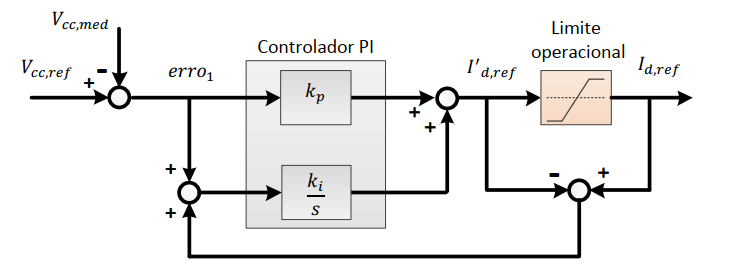
\includegraphics[width=\columnwidth]{figuras/Malha_Anti_Windup.PNG}
			% Create a subtitle for the figure.
			\caption{Malha de controle Anti Windup. Fonte: \cite{TeseProfAlex}}
			% Define the label of the figure. It's good to use 'fig:title', so you know that the label belongs to a figure.
			\label{fig:Malha_anti_windup}
		\end{center}
	\end{figure}
	
	
\end{itemize}

As referências finais para as malhas de controle de corrente, representadas pela corrente de eixo direto $I_{d,ref}$ e  e de eixo em quadratura $I_{q,ref}$ são comparadas com as mesmas grandezas resultantes da medição. A diferença que existe entre estas, ou o erro, é submetido, respectivamente, aos controladores PI-2 e PI-4, que são responsáveis por gerar os valores de referência para as tensões de eixo direto $V_d$ e de eixo em quadratura $V_q$. É importante salientar a inserção dos termos referentes ao acoplamento entre as malhas de controle como parcelas \textit{feedforward}, conforme proposto por \cite{astrom2006advanced}, cujas variáveis de saída são as tensões de eixo direto $E_d$ e de eixo em quadratura $E_q$, a serem sintetizadas nos terminais de saída do inversor. 

\section{Sistema de Medição e Transformação de Grandezas}

É necessário ainda comentar sobre o mecanismo de transformação das grandezas medidas necessárias para a estratégia de controle, que podem ser visualizadas na Fig. \ref{fig:Estrategia_Grandezas}. Destaca-se o uso da Transformada de Park para o cálculo da potência instantânea, a qual é calculada a partir das variáveis de eixo direto e de eixo em quadratura.

\begin{figure}[!hbt]
	% Center the figure.
	\begin{center}
		% Include the eps file, scale it such that it's width equals the column width. You can also put width=8cm for example...
		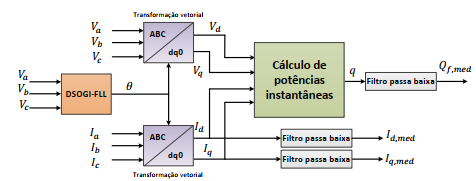
\includegraphics[width=\columnwidth]{figuras/Transformacao_Grandezas.PNG}
		% Create a subtitle for the figure.
		\caption{Estratégia de transformação de grandezas e cálculo da potência reativa. Fonte: \cite{TeseProfAlex}}
		% Define the label of the figure. It's good to use 'fig:title', so you know that the label belongs to a figure.
		\label{fig:Estrategia_Grandezas}
	\end{center}
\end{figure}

Pode-se visualizar na Fig. \ref{fig:Estrategia_Grandezas} que as tensões no ponto de acoplamento são utilizadas como variáveis de entrada para a estrutura \textit{Frequency Locked Loop} (FLL). A estrutura da FLL será discutida posteriormente neste trabalho, mas convém destacar neste momento que esta tem por objetivo produzir o ângulo de fase das tensões $\theta $, de forma que se realize a transformação vetorial de tensões e correntes. De forma a converter as grandezas de fase (a, b e c) em grandezas de eixo direto e de eixo em quadratura (d e q), utiliza-se a matriz de transformação $T_{dq}$, conforme as Eqs. \ref{eq:matrix_transformacao} e \ref{eq:matriz_transformacao_2}. As variáveis de eixo direto e de eixo em quadratura das correntes a, b e c também são obtidas por equações similares.

\begin{align}
V_{dq} = [T_{dq}][V_{\alpha \beta}]\nonumber
\end{align}

\begin{align}\label{eq:matrix_transformacao}
\begin{bmatrix}
	V_d \\ V_q
\end{bmatrix} = 
\begin{bmatrix}
	\cos{\theta} & \sin{\theta} \\
	-\sin{\theta} & \cos{\theta}
\end{bmatrix}
\begin{bmatrix}
	v_{\alpha} \\ v_{\beta}
\end{bmatrix}
\end{align}

\begin{align}\label{eq:matriz_transformacao_2}
	\begin{bmatrix}
		v_d \\ v_q
	\end{bmatrix} = \frac{2}{3}
	\begin{bmatrix}
		\cos{\theta} & \cos(\theta - \frac{2\pi}{3}) & \cos(\theta + \frac{2\pi}{3}) \\
		-\sin{\theta} & -\sin(\theta - \frac{2\pi}{3}) & -\sin(\theta + \frac{2\pi}{3}) \\
	\end{bmatrix}
	\begin{bmatrix}
		v_a \\ v_b \\ v_c
	\end{bmatrix}
\end{align}

Utilizando os resultados obtidos, obtêm-se a potência reativa medida $q$, cujo cálculo é realizado conforme a Eq. \ref{eq:potencia_reativa_medida}.

\begin{align}\label{eq:potencia_reativa_medida}
	q = \frac{3}{2}(V_d I_q - V_q I_d)
\end{align}

Devido aos desequilíbrios e distorções harmônicas existentes nas variáveis medidas, realiza-se um processo de filtragem do sinal obtido. Mais especificamente, filtros do tipo \textit{Butterworth} de 1ª ordem foram utilizados, com frequência de corte definida em 100 rad/s. O mesmo procedimento foi utilizado para as correntes de eixo direto e em quadratura, onde estas foram submetidas à um filtro do tipo \textit{Butterworth} de 1ª ordem com frequência de corte de 500 rad/s.

\section{Método de Sincronismo}

Quando deseja-se integrar fontes eólicas à rede elétrica, em destaque para as que utilizam conversores para o processamento da energia produzida, deve-se realizar a sincronização das tensões sintetizadas pelo inversor com aquelas existentes no ponto de acoplamento \cite{TeseProfAlex}. 

Além disso, pertubações de rede levam a problemas de qualidade de energia, como desbalanceamento de tensão, quedas/picos de tensão, flutuações de tensão, faltas de fase e inserção de harmônicos indesejáveis em sistemas conectados à rede. Dessa forma, um método apropriado de sincronização é requerido para superar estes problemas \cite{Meral2018}. 

Baseado nestes aspectos, o uso de estruturas de detecção de módulo e ângulo de fase de tensões trifásicas, como a tecnologia denominada \textit{Frequency Locked Loop} - FLL, é decisivo para que o fluxo de energia ativa e reativa não ocasione instabilidades no sistema elétrico.

De forma que os requisitos estabelecidos sejam cumpridos, neste trabalho é utilizado umas das técnicas mais difundidas na literatura tratando-se da sincronização de inversores com a rede elétrica, conhecida como \textit{Dual Second-Order Generalized Integrator FLL} (DSOGI-FLL), cujo diagrama de bloco é apresentado na Fig. \ref{fig:DSOGI_FLL}.  

\begin{figure}[!hbt]
	% Center the figure.
	\begin{center}
		% Include the eps file, scale it such that it's width equals the column width. You can also put width=8cm for example...
		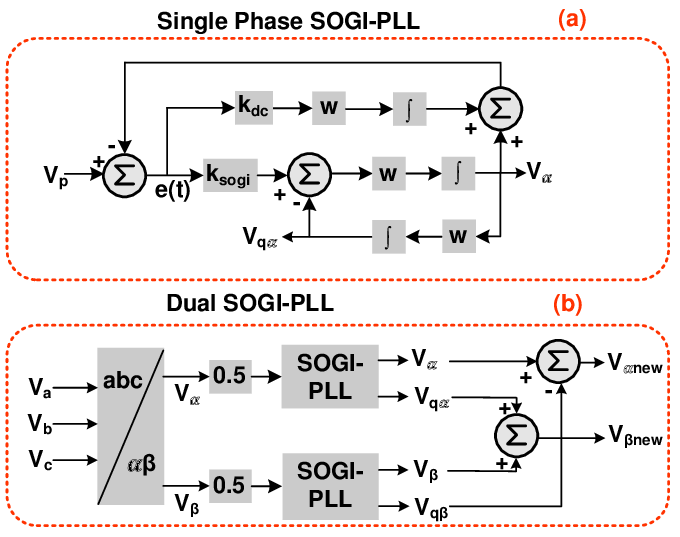
\includegraphics[width=\columnwidth]{figuras/DSOGI_PLL.PNG}
		% Create a subtitle for the figure.
		\caption{Diagrama de blocos completo do DSOGI-FLL. Fonte: \cite{DissertacaoJoao}}
		% Define the label of the figure. It's good to use 'fig:title', so you know that the label belongs to a figure.
		\label{fig:DSOGI_FLL}
	\end{center}
\end{figure}

O DSOGI-FLL é uma metodologia que cumpre os requisitos de sincronismo com a rede elétrica e tem como vantagens simplicidade estrutural, facilidade de implementação, rejeição de distorções harmônicas e desequilíbrios, precisão na extração da sequência positiva, adaptabilidade a possíveis variações na frequência nas tensões da rede e precisão do ângulo calculado. A posição angular e a frequência na saída da FLL são utilizadas na transformações de Park das correntes medidas, possibilitando assim a realização da estratégia de controle do inversor de frequência \cite{DissertacaoJoao}.

Os aspectos da modelagem matemática desta estrutura e sua respectiva análise de desempenho fogem do escopo e não serão apresentados neste trabalho, porém podem ser verificados com detalhes nos trabalhos de \cite{ArticleRodriguez} e \cite{book-remusteodorescu201b1}.


\section{Modulação por Largura de Pulso - PWM}


\subsection{Modulação por Largura de Pulso Senoidal - SPWM}


\section{Aquisição e Condicionamento de Sinais de Corrente e Tensão}

A etapa de aquisição e condicionamento de sinais destina-se à obtenção de tensões e correntes no ponto de conexão do inversor, e tem o objetivo entregar os parâmetros necessários para o algoritmo de controle realizado no microcontrolador. 

O sistema de aquisição e condicionamento de sinais é constituído pelos seguintes componentes:

\begin{itemize}
	\item Sensores de tensão e corrente;
	\item Filtros \textit{anti-aliasing};
	\item Circuitos de tratamento de sinal (somadores e reguladores de tensão)
\end{itemize}

\subsection{Transdutor de Tensão}

\subsection{Filtro Anti-Aliasing}

	Uma vez realizada a aquisição dos sinais de interesse, estes devem estar adequados para que sua manipulação por meio do microcontrolador seja possível. A rede elétrica possui diversos ruídos e transitórios eletromagnéticos de alta frequência que podem interferir no sinal de interesse (COLOCAR REFERÊNCIA), de modo que é necessário realizar uma filtragem analógica destas harmônicas indesejáveis anteriores ao microcontrolador.
	
	Desta forma, é utilizado na placa de aquisições um filtro \textit{butterworth} passa-baixas de 1ª ordem, com frequência de corte de 234 Hz. A topologia deste filtro é apresentada na Figura \ref{fig:filtro-butter}.
	
\begin{figure}[!hbt]
         % Center the figure.
         \begin{center}
         % Include the eps file, scale it such that it's width equals the column width. You can also put width=8cm for example...
         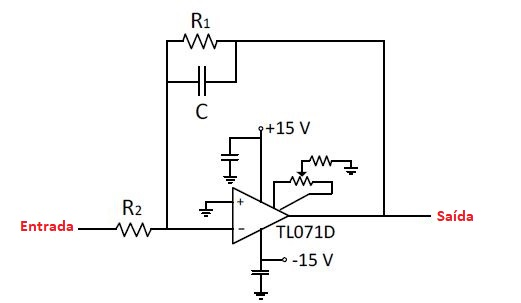
\includegraphics[scale=0.7]{figuras/filtro-butter.JPG}
         % Create a subtitle for the figure.
         \caption{Topologia do filtro de Butterworth de primeira ordem utilizado na placa de condicionamento de sinais}
         % Define the label of the figure. It's good to use 'fig:title', so you know that the label belongs to a figure.
         \label{fig:filtro-butter}
         \end{center}
 \end{figure}


	A frequência de corte deste filtro é dado pela Eq. 
	
\begin{align}
	f_{co} = \frac{1}{2\pi R_1 C} \label{eq:freq_corte_butter} \\
	K = -\frac{R_2}{R_1}\label{eq:ganho_butter}
\end{align}

\subsection{Circuito Somador}

Um circuito com amplificador operacional na topologia de somador é necessário para que se adicione um nível DC ao sinal proviniente do filtro \textit{anti-aliasing}, de forma que o sinal a ser amostrado reproduza apenas valores positivos e compatíveis com os limites de tensão do conversor A/D do microcontrolador. 

A topologia escolhida foi a de \textbf{somador não-inversor}, pois este não altera os ângulos de fase dos sinais provenientes dos transdutores. A Figura \ref{fig:somador-ninversor} mostra o circuito do somador não inversor. A equação que relaciona a tensão de saída com as tensões de entrada são dadas pela Eq. \ref{eq:circuito-somador}, onde $V_{REF}$ é a tensão de nível CC que é somada ao sinal que vem do filtro anti-aliasing, $V_1$.

\begin{align}
	V_{out} = \left(1+\frac{R_a}{R_b}\right)\left(\frac{V_1/R_1 + V_{REF}/R_2}{1/R_1 + 1/R_2}\right)\label{eq:circuito-somador}
\end{align}

\begin{figure}[!hbt]
	% Center the figure.
	\begin{center}
		% Include the eps file, scale it such that it's width equals the column width. You can also put width=8cm for example...
		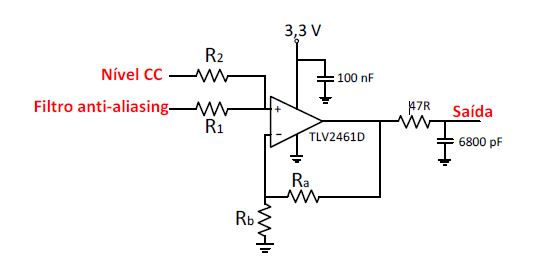
\includegraphics[scale=0.7]{figuras/somador-ninversor.JPG}
		% Create a subtitle for the figure.
		\caption{Circuito somador não-inversor}
		% Define the label of the figure. It's good to use 'fig:title', so you know that the label belongs to a figure.
		\label{fig:somador-ninversor}
	\end{center}
\end{figure}

\subsubsection{Circuito de fornecimento de tensão CC}

Um outro circuito, anterior ao somador é utilizado para fornecer tensão CC regulável ao somador, de forma que está possa estar dentro dos limites estabelecidos pelo microcontrolador. A Figura \ref{fig:divisor-tensao} mostra a topologia do circuito. A resistência variável conectada ao amplificador operacional permite o ajuste fino do divisor de tensão.

\begin{figure}[!hbt]
	% Center the figure.
	\begin{center}
		% Include the eps file, scale it such that it's width equals the column width. You can also put width=8cm for example...
		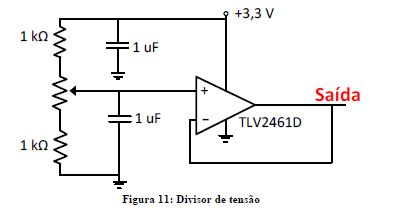
\includegraphics[scale=0.7]{figuras/divisor-tensao.JPG}
		% Create a subtitle for the figure.
		\caption{Divisor de tensão com resistência variável}
		% Define the label of the figure. It's good to use 'fig:title', so you know that the label belongs to a figure.
		\label{fig:divisor-tensao}
	\end{center}
\end{figure}

\subsection{Circuito Regulador de Tensão}

O circuito de regulação e filtragem de tensão destina-se ao suprimento de tensão aos amplificadores operacionais e transdutores da placa de aquisição. A Figura \ref{fig:circuito-regulacao} mostra os componentes deste circuito. Este é basicamente composto por \textit{beads} de ferrite e capacitores destinados à minimização de ruídos existentes na tensão de suprimento da placa. A placa de aquisição de sinais é alimentada por uma fonte externa que deve dispor de tensões contínuas de +15 V e -15 V.

\begin{figure}[!hbt]
	% Center the figure.
	\begin{center}
		% Include the eps file, scale it such that it's width equals the column width. You can also put width=8cm for example...
		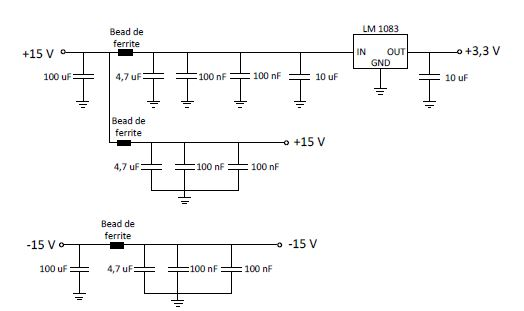
\includegraphics[scale=0.7]{figuras/circuito-regulador.JPG}
		% Create a subtitle for the figure.
		\caption{Circuito para regulação e filtragem de tensão}
		% Define the label of the figure. It's good to use 'fig:title', so you know that the label belongs to a figure.
		\label{fig:circuito-regulacao}
	\end{center}
\end{figure}


